\providecommand{\main}{..}
\documentclass[../mthe-493-final-project.tex]{subfiles}

% Overall implementation of our design solution.
\begin{document}
    \chapter{Implementation}
    \label{ch:implementation}

    \section{Distributed Computing}
    \label{sec:distributed-computing-implementation}

    % "Performs an economic analysis on multiple solutions and uses quantitative justification when choosing solution"
    \subsection{Tool Selection}
    
    While the optimization portion of the design was being implemented, the team decided to move forward with implementing the distributed computing portion of the design solution using Axon. The decision came down to two main reasons: ease in implementing the cost structure and the lower overall economical cost.

    As mentioned in~\autoref{subsec-ete-evaluation-of-tools}, DCP's cost structure between clients and workers has the downside of having clients paying a set amount decided at the beginning of work distribution. If it were to be used in the implementation of the design solution, we would need to spend additional time and resources working with Kings Distributed Systems to create a non-trivial workaround. On the other hand, Axon's lack of a cost structure means that the team would also need to spend time implementing the cost structure from scratch. Working with Duncan would save time on implementing a cost structure, and meeting the problem description's requirements would be simpler than trying to build on top of an already complex cost structure on DCP. Thus, Axon became the clear choice in terms of lower time cost and lower complexity without trading off accuracy for the purposes of the design solution.

    Another aspect of DCP that comes from it being more of a commercial product rather than a pure research tool is the cost of using the tool in practice. According to their website and when one attempts to buy credits to deploy work on DCP, It costs around \$100 to access approximately a years worth of virtual CPU computational time~\cite{kings-ds-marketing}. On the other hand, implementing the design solution in practice using Axon doesn't have a similar cost~\cite{Mays_Axon}. Based on that, Axon also becomes the preferred choice in terms of economic cost.
    
    \subsection{Network Architecture}
    \label{ssec:network-architecture}
    % Description of approach and final code-base architecture. Our physical model. Great place for an architecture diagram.
    % Naive translation form math model to actual implementation.
    % e.g., workers are represented as machines on a network

    With the distributed computing framework chosen, the team then designed how the cost structure, optimization algorithm, and parallel learning components were going to fit into network connecting the orchestrator to the learners.

    A disclaimer regarding terminology: both the distributed computing frameworks, DCP and Axon, use the term \textit{worker} to represent a \textit{learner}~\cite{Mays_Axon}\cite{noauthor_worker_nodate}. Axon uses the term \textit{client} to represent an \textit{orchestrator}~\cite{Mays_Axon}. As such, the rest of the section will use the former terms mentioned to refer to the network nodes.

    The first task to implement the network was ensuring that the client can communicate with the workers. In Axon, the intended method of doing that programmatically is through a ``noticeboard''. It works by having workers that start up sign in to the notice board to be discovered. Then when a client connects to the noticeboard to discover them, it responds with the workers that have signed in~\cite{Mays_Axon}.

    An overview of the network nodes and their relationships can be observed in~\autoref{fig:network-flowchart}.
    
    \begin{figure}
        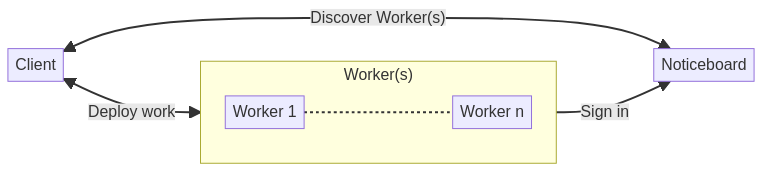
\includegraphics{network-1.png}
        \caption{Flowchart diagram of the network's architecture~\cite{group_a2_Optimization_Of_Data}.}
        \label{fig:network-flowchart}
    \end{figure}

    As far as what computers the entity's were located on, the discussion on raspberry pis versus personal computers in~\autoref{subsec-ete-evaluation-of-tools} contributed to the experimental set up involving running the nodes on personal computers for their hardware's capability to run the parallel learning tasks. Running node on a computer equates to starting python scripts as programs that can send and receive messages over their computer's local network. For simplicity, the client and noticeboard programs were ran on the same computer since the noticeboard was not computationally demanding for the small network sizes being used during experimentation. Naturally, workers are started on other computers on the local network.

    With the overall architecture of the network finalized, the team then implemented each of the sub components of the design solution pertaining to important steps that occur during an experiment, which can be observed in~\autoref{fig:network-sequence}.

    \begin{figure}
        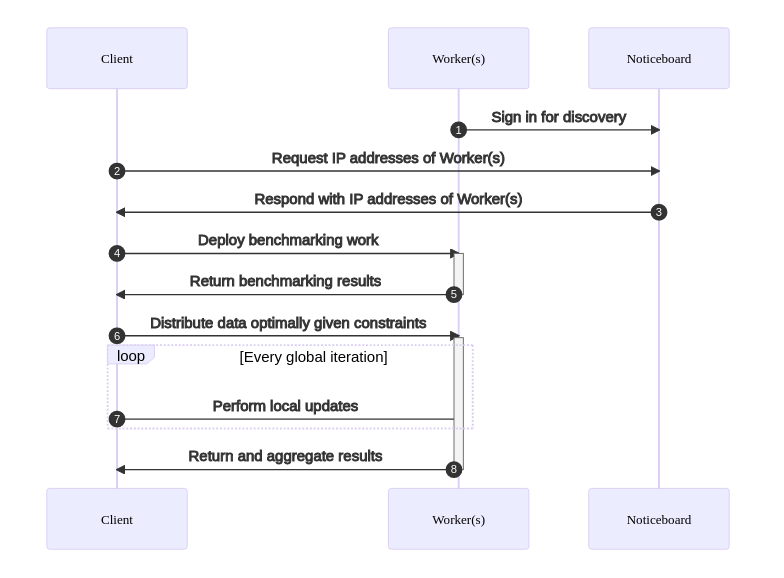
\includegraphics{network-2.png}
        \caption{Sequence diagram of an experiment~\cite{group_a2_Optimization_Of_Data}.}
        \label{fig:network-sequence}
    \end{figure}

    Steps 1 and 2 from the figure describe how the client connects to the workers mentioned earlier more precisely. The rest of the steps will form the basis of what will be discussed next in the implementation.

    But an aspect of the system that isn't shown in the sequence diagram is the cost structure. After the client discovers the workers, the teams implemented the feature by designing the client to have the ability to set each worker's recruitment cost. In a more realistic set up, each worker would set their recruitment costs, with some thought given to each of their computational capabilities. This design decision came from a need to make setting up test cases for experiments easier. Instead of spending time setting up a system to update the recruitment cost of each worker on the network outside of the client, it would be simpler to send each worker their recruitment cost from the client once they are connected~\cite{group_a2_Optimization_Of_Data}. 

    \subsection{Benchmarking}
    \label{ssec:benchmarking}

    The next step after the client and workers have connected and set the recruitment costs is to have the client determine the computational capabilities of each worker, i.e., steps 4 and 5 from~\autoref{fig:network-sequence}. To do so, the client sends each worker work that calculates their computational capabilities, work that Duncan Mays has provided to the team~\cite{mays_benchmark_nodate}.

    As specified by Duncan's work, each learner $l_i$ will be benchmarked to estimate a \textit{sample compute rate}, $C_i$. Each learner also has a \textit{fee} to compute a sample, $r_i$. We can define the quantity:
    
    \textit{Subjob compute time}, $t^c_i$, which is a function of $s_i$
                  \[t^c_i = \frac{\tau s_i}{C_i}\]

    The upper bound on training time yields an inequality

    \[t^c_i < T \quad \forall w_i \in \mathbf{W}.\]

    from which an upper bound on \textit{subjob size} is derived

    \[s^{max}_i < \frac{T C_i}{\tau}.\]

    The implementation uses the benchmarking job provided by Duncan to determine $s^{max}_i$~\cite{group_a2_Optimization_Of_Data}\cite{mays_benchmark_nodate}.

    After the client receives the benchmarking results, the optimization in the next step (step 6) seen in~\autoref{fig:network-sequence} can occur which will be discussed next.
    
    \section{Optimization}
    \label{sec:optimization-implementation}
    
    Implementation of the optimization portion of the project was focused on creating a modular interface for the orchestrator to use when data is to be assigned to learners. Assumptions about the orchestrator's interface, the architecture, and implementation details are presented below.
    
    \subsection{Orchestrator Interface}
    \label{ssec:optimization-orchestrator-interface}
    
    The interface was designed assuming that the orchestrator calls the \texttt{assign\_work} routine of an \texttt{Optimizer}, providing arguments for
    
    \begin{itemize}
        \item the data set $D$ of homogeneous batches of training data;
        \item the set of learners (workers) $\mathbf{L}$, each with properties describing
        \begin{itemize}
            \item their ID,
            \item their cost per batch of data, $c_i$,
            \item their maximum assigned work, $s^{max}_i$, and
            \item the set slices assigned to it, $D_i$, which is initially empty;
        \end{itemize}
        \item the system parameters $\beta$ and $s^{min}$.
    \end{itemize}
    
    It is then the task of the \texttt{Optimizer} to determine if the problem is feasible, and if so, set the $D_i$ property of each worker according to the MIP problem as defined in \autoref{sec:optimization-problem-description}.
    
    \subsection{Architecture}
    \label{ssec:optimization-architecture-implementation}
    
    The architecture was designed to comply with the specifications set during in tool selection (\autoref{sec:optimization-engineering-tools}) alongside the above assumptions. To accommodate both the Gurobi optimizer and heuristic algorithm, and to generalize the interface such that other optimizers may be implemented, the \texttt{Optimizer} class was created as the primary interface with which the orchestrator will interact. This encapsulates the general behaviour of an optimizer within the system: an optimizer assesses whether the problem is feasible given the aforementioned parameters. If so, slices are assigned to workers. If not, a \texttt{DataAssignmentError} is thrown (raised) to indicate the optimization problem is infeasible. This is depicted in \autoref{fig:optimization-architecture}.
    
    \begin{figure}
        \centering
        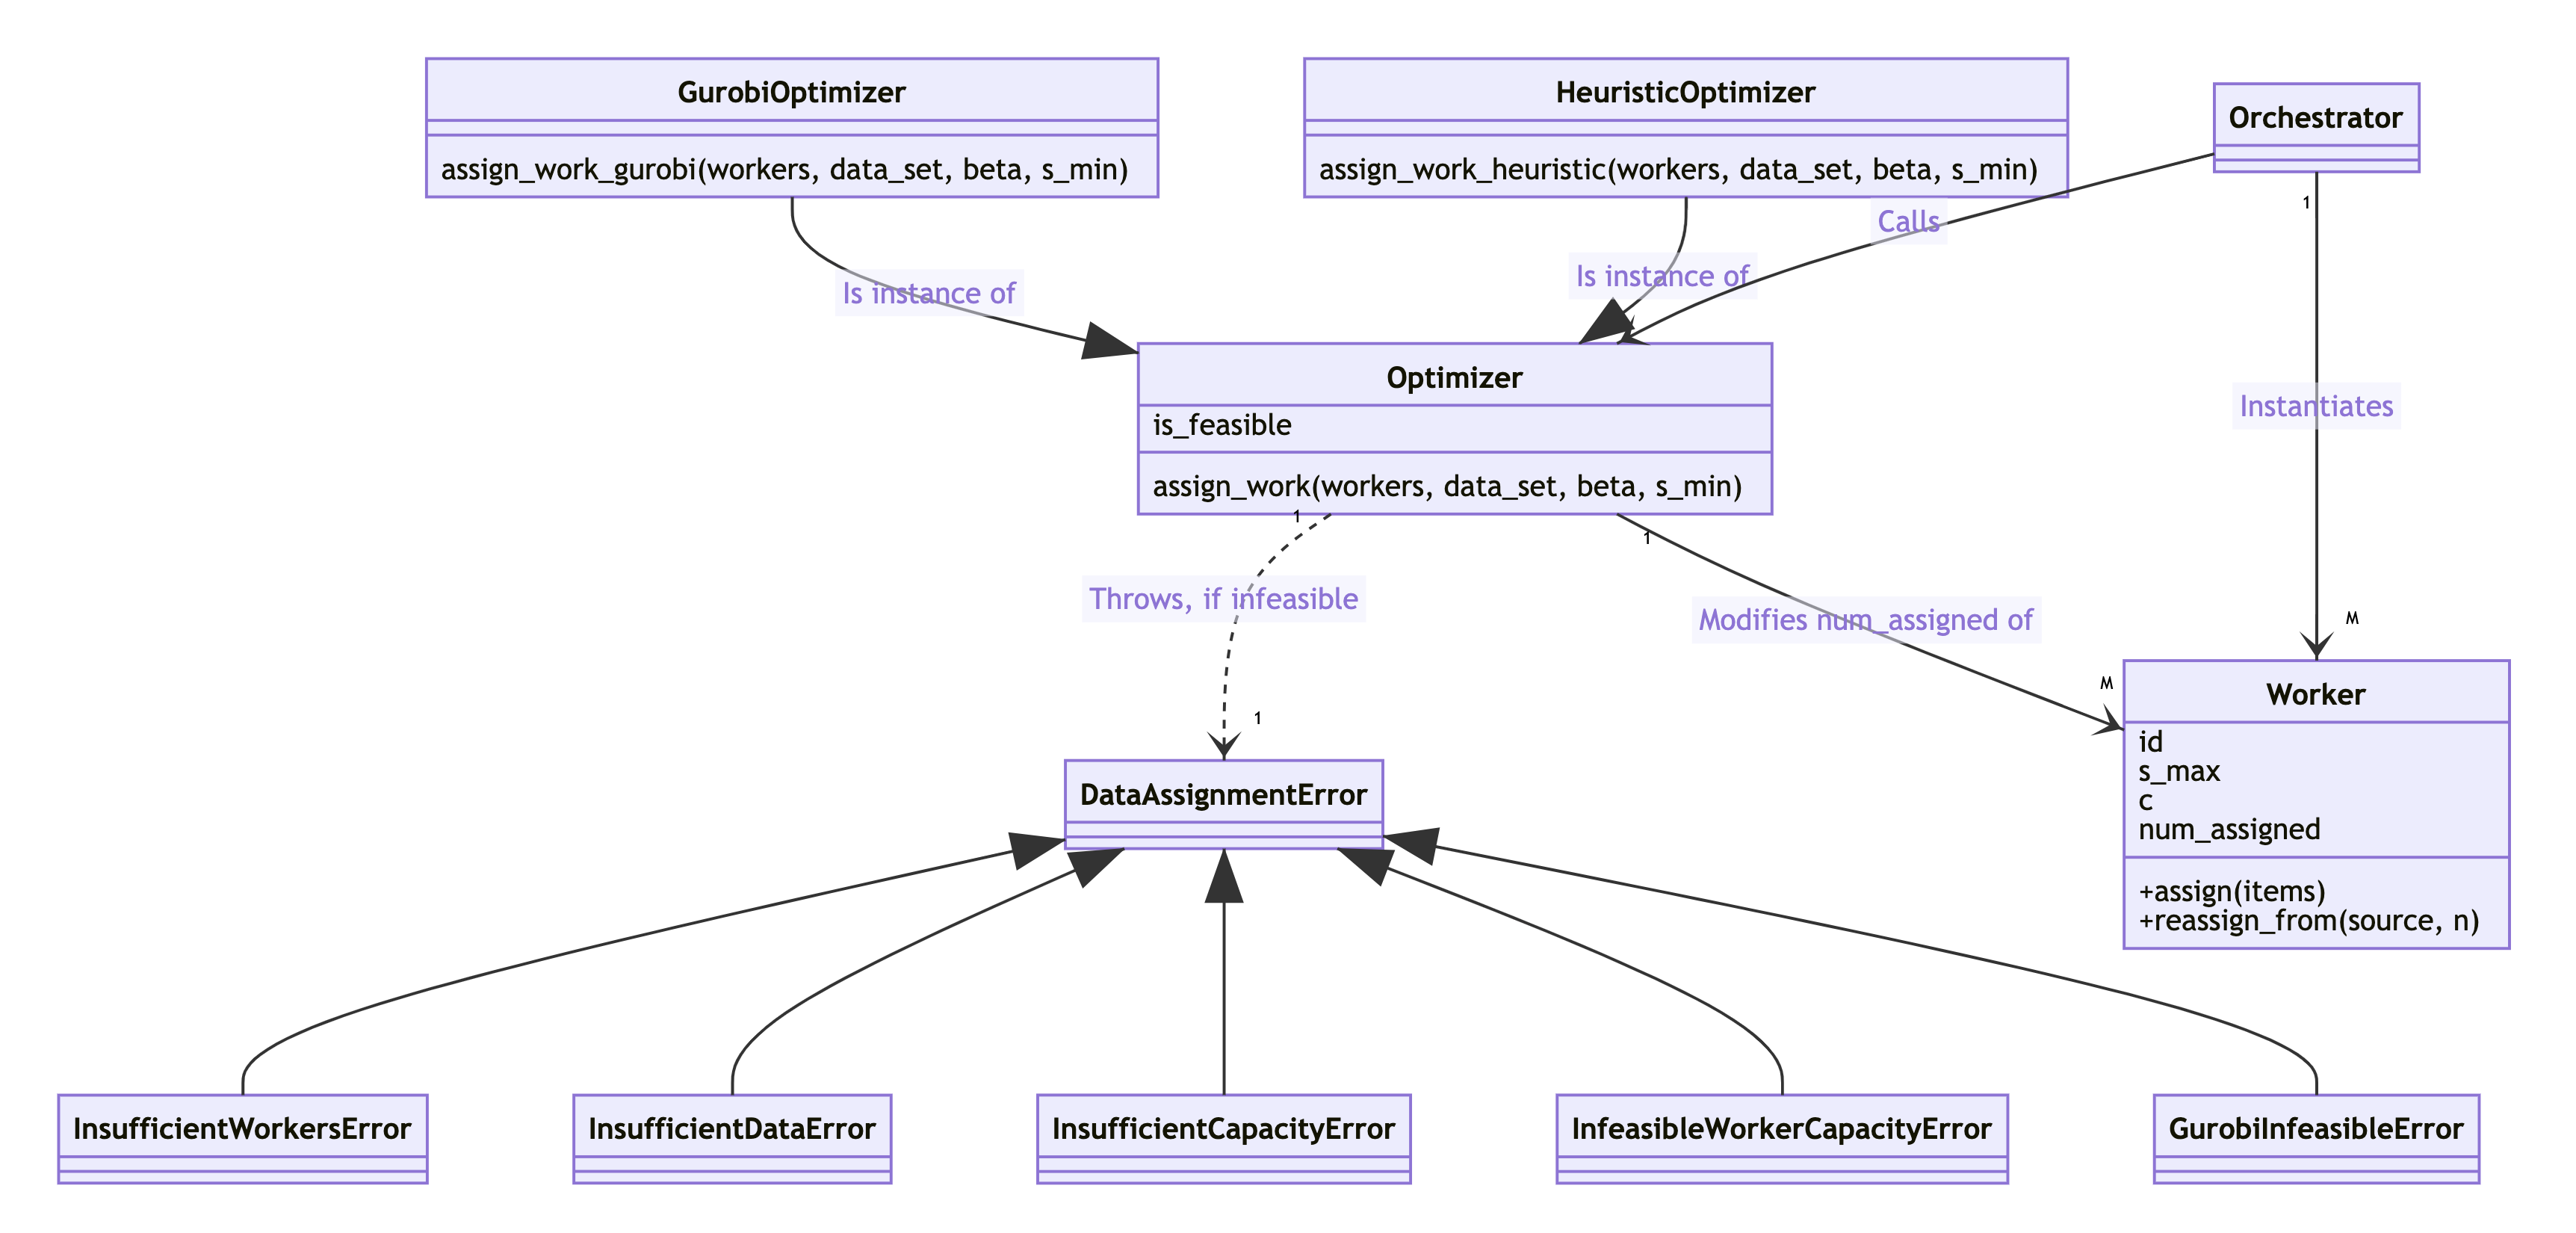
\includegraphics{thesis/img/data_assignment.png}
        \caption{Architecture diagram of optimization implementation}
        \label{fig:optimization-architecture}
    \end{figure}
    
    In this model, the \texttt{GurobiOptimizer} represents the implementation of the Gurobi optimization solver, and \texttt{HeuristicOptimizer} represents the implementation of the heuristic algorithm. Both are instances of an \texttt{Optimizer}, meaning they both implement the same high-level functionality from the perspective of the orchestrator.
    
    Besides the obvious differences in how each optimizer determines the partition $\boldsymbol{D}$ of $D$, they also differ in the resolution of response that is provided in the case of an infeasible optimization problem.
    
    \subsection{\texttt{GurobiOptimizer}}
    \label{ssec:optimization-gurobi-optimizer-implementation}
    
    The \texttt{GurobiOptimizer} implements the MIP problem with Gurobi as stated in \autoref{ssec:optimization-problem-simplification}, i.e. including the simplifications on constraints from \eqref{eq:simplified-optimization-constraint-1} and \eqref{eq:simplified-optimization-constraint-3}. A simple check after running the solver checks whether the problem is feasible.
    
    If the problem is feasible, each learner is assigned the optimal subset $D_i \subseteq D$ according to the value of $x_i$ determined by the solver. If the problem is infeasible, a \texttt{GurobiInfeasibleError} (an instance of \texttt{DataAssignmentError}) is thrown.
    
    Herein lies the limitation in infeasible response alluded to above: \texttt{GurobiOptimizer} is only capable of indicating that a problem \textit{is} or \textit{is not} feasible, but cannot provide suggestions as to \textit{why} a problem is infeasible. Oftentimes a simple misconfiguration of system parameters ($\beta$ or $s_{min}$) result in infeasibility, but there is no way to detect this when using this optimizer. This is a result of Gurobi not understanding the semantics of the MIP problem; this is a clear disadvantage to this optimizer.
    
    \subsection{\texttt{HeuristicOptimizer}}
    \label{ssec:optimization-heuristic-optimizer-implementation}
    
    The \texttt{HeuristicOptimizer} implements a heuristic algorithm which is capable of solving the MIP problem as stated in \autoref{sec:optimization-problem-description}.
    
    The algorithm includes distinct checks at multiple stages to ensure the problem is feasible for various reasons. This provides a better understanding to the user over why a given system is deemed infeasible, which is a clear advantage over the \texttt{GurobiOptimizer}. 
    
    \subsubsection{Heuristic Algorithm}
    \label{sssec:optimization-heuristic-algorithm}
    
    For clarity, the algorithm is presented, followed by a summary of the purpose of each step. The algorithm is consists of the following steps:
    
    \begin{enumerate}
        \item Inputs $D$, $\mathbf{L}$, $\beta$, $s^{min}$ as stated in \autoref{ssec:optimization-orchestrator-interface}.
        \item Let $n := \vert D \vert$, $k := \vert \mathbf{L} \vert$
        \item Assume WLOG: $n > 0$; $k > 0$; $s^{min} > 0$; $\beta > 0$. 
            \begin{enumerate}
                \item If assumption(s) fail, \textbf{raise} a general \texttt{ValueError}
            \end{enumerate}
        \item Check $n \geq \beta \cdot s^{min}$
            \begin{enumerate}
                \item If false, \textbf{raise} \texttt{InsufficientDataError}
            \end{enumerate}
        \item Let $k_{max} := \lfloor \frac{n}{s^{min}} \rfloor$ be the \textit{maximum number of employable workers}
        \item Find $\mathbf{L}_e \subseteq \mathbf{L}$, the \textit{subset employable workers}:
            \begin{enumerate}
                \item Set $\mathbf{L}_e := \{ l_i \in \mathbf{L} : s^{max}_i \geq s^{min} \}$
                \item Let $k_e := \vert \mathbf{L}_e \vert$
                \item Reorder indices of $l_i \in \mathbf{L}_e$ such that $c_1 < c_2 < ... < c_{k_e}$
                \item If $k_e \leq k_{max}$, go to Step 7
                \item Let $\mathbf{L}_e^{all} := {\mathbf{L}_e \choose k_{max}}$ be the set of combinations of $\mathbf{L}_e$ of length $k_{max}$ in \textit{lexicographical order} given by the indices $i, \ \forall \ l_i \in \mathbf{L}_e$, and denote by $N$ the size of $\mathbf{L}_e^{all}$
                \item For $j := 1, ..., N$:
                    \begin{enumerate}
                        \item Set $\mathbf{L}_e := \left( \mathbf{L}_e^{all} \right)_j$
                        \item If $\sum_{l_i \in \mathbf{L}_e} s^{max}_i \geq n$, go to Step 7
                    \end{enumerate}
                \item If no combination meets requisite capacity, \textbf{raise} \texttt{InfeasibleWorkerCapacityError}
            \end{enumerate}
        \item Check $k_e \geq \beta$
            \begin{enumerate}
                \item If false, \textbf{raise} \texttt{InsufficientWorkersError}
            \end{enumerate}
        \item Check $\sum_{l_i \in \mathbf{L}_e} s^{max}_i \geq n$.
            \begin{enumerate}
                \item If false, \textbf{raise} \texttt{InsufficientCapacityError}
            \end{enumerate}
        \item Let $n_{assigned} := 0$; $i^{last} := 1$
        \item Repeat while $n_{assigned} < n$:
            \begin{enumerate}
                \item Let $l_i := \left( \mathbf{L}_e \right)_{i^{last}}$; $x_i := \min\{s^{max}_i, n - n_{assigned}\}$
                \item Assign the next $x_i$ elements of $D$ to $l_i$
                \item Update $n_{assigned} := n_{assigned} + x_i$
                \item If $x_i \geq s^{min}$, set $i^{last} := i^{last} + 1$
            \end{enumerate}
        \item Let $k_{assigned} := i^{last} + 1$
        \item Repeat up to $k_e - i^{last}$ times:
            \begin{enumerate}
                \item Let $k_{complete} := \vert \{l_i \in \mathbf{L}_e : x_i \geq s^{min} \} \vert$
                \item If $k_{complete} \geq \max\{\beta, k_{assigned}\}$, return \textbf{Success}
                \item Reassign $\max\{0, s^{min} - x_{i^{last}}\}$ batches to learner $l_{i^{last}}$ from learners $\{l_1, ..., l_{k_{complete}}\}$, taking \textit{at most} $x_j - s^{min}$ from learner $l_j$, for $j = k_{complete}, k_{complete} - 1, ..., 1$
                \item Set $i^{last} := i^{last} + 1$
            \end{enumerate}
    \end{enumerate}
    
    \begin{itemize}
        \item \textbf{Steps 1-2} defines inputs and derived properties
        \item \textbf{Step 3} asserts that key properties are positive, otherwise the problem is infeasible
        \item \textbf{Step 4} ensures the actual data set size meets or exceeds the implied data set size from the values of $\beta$ and $s^{min}$
        \item \textbf{Step 5} defines \textit{maximum number of employable learners}, $k_{max}$. This is a crucial value in determining feasibility when $s^{min}$ is relatively large compared to $n$. E.g. if $s^{min} = 100$ and $n = 350$, \textit{at most} 3 learners can be employed, regardless of $k$.
        \item \textbf{Step 6} finds a subset of \textit{employable learners} and orders them in ascending order of cost. Employable learners must have $s^{max}_i \geq s^{min}$. If the number of employable learners is greater than $k_{max}$, we must find a subset of learners of length $k_{max}$ that has the capacity to compute $D$. Building on the previous example, if $k = 10$ and $100 \leq s^{max}_i \leq 115 \ \forall i$, then the problem is infeasible because no subset of 3 learners can compute a data set of $n = 350$.
        \item \textbf{Step 6(e)} has some room for improvement. The usage of lexicographical ordering does not guarantee the \textit{optimal} subset of learners is chosen. This is a trade-off for better speed at the cost of reduced accuracy.
        \item \textbf{Steps 7-8} check that constraints \eqref{eq:simplified-optimization-constraint-1} and \eqref{eq:simplified-optimization-constraint-2} can be satisfied, respectively.
        \item \textbf{Steps 9-10} setup and perform the \textit{initial assignment phase}, wherein the entire data set is assigned to the cheapest learners until no more data can be assigned
        \item \textbf{Steps 11-12} setup and perform the \textit{reassignment phase}. This corrects any incomplete learners (those who were assigned some data, but less than $s^{min}$ data), and ensures the beta constraint is actually met. This involves reassigning as many batches as possible from the most expensive learners \textit{who have more than $s^{min}$ data} to incomplete workers until all constraints are met.
    \end{itemize}
    
    \subsubsection{Suboptimality of Heuristic Algorithm}
    \label{sssection:optimization-heuristic-suboptimality}
    
    An earlier version of the problem definition without the $s^{min}$ constraint from \eqref{eq:optimization-constraint-1} (or rather, $s^{min}$ was always assumed to be 1) was proved to be optimal with a similar (but much simpler) algorithm. The earlier version did not require the use of \textbf{Step 6}, and thus did not contain any sub-optimal steps. In contrast, this algorithm is suboptimal because \textbf{Step 6(e)} does not always select the minimum-cost subset of employable workers. This manifests during the \textit{reassignment phase}, where it is possible that the algorithm reassigns to more workers than is necessary, resulting in a marginally increased cost over the optimal solution
    
    \subsection{Evaluation of Optimizer Implementations}
    \label{ssection:optimization-optimizer-implementation-evaluation}
    
    As noted in \autoref{ssec:optimization-tool-selection}, the \texttt{HeuristicOptimizer} would need to be compared to the alternative \texttt{GurobiOptimizer}. This was accomplished through an extensive testing suite and logging system, which included:
    
    \begin{itemize}
        \item A \textit{test case generator} with seeded randomness and user-controlled parameter ranges. This allows the user to generate any number of test cases in a deterministic fashion for reproducibility, whilst allowing parameter ranges (number of workers, costs, maximum assigned data, data set size, $\beta$, $s^{min}$) to be selected.
        \item A \textit{test set runner}, which runs a set of test cases using a given \texttt{Optimizer}, parses, collects, and aggregates performance and timing metrics of the optimizers under the tests.
        \item A \textit{optimizer test comparator} that combines the generator and runner by producing two identical test sets, executing them with the runner for two different \texttt{Optimizer}s, and comparing the results on every individual test case. This outputs key metrics about whether the optimizers agreed on feasibility and optimal minimum cost, alongside best- and worst-case running time analyses.
    \end{itemize}
    
    These tools were used extensively during the development of both the \texttt{HeuristicOptimizer} and \texttt{GurobiOptimizer} to ensure both were working correctly, to discover limitations, and to assess optimizer running times.

    \section{Parallel Learning}
    \label{sec:parallel-learning-impl}
    Tool selection for the parallel learning portion of our problem was nontrivial. All three of the papers that were evaluated earlier had their upsides, but only one of the methods could reasonably be implemented due to the scope and duration of our project. The first paper to be dropped from consideration for our project’s use case was FedProx. At the time the decision was made, our proposed network of learners was to consist of almost entirely raspberry pis. This meant all of our experimental results would be collected with little to no system heterogeneity. Seeing as FedProx’s main advantage over FedAvg came in highly heterogenous settings, it made very little sense for our group to implement this aggregation technique. 

    This left a choice between FedAvg, the gold standard in model aggregation, and q-FedAvg, a potentially more efficient version of FedAvg. Although the efficiency and expedited convergence that q-FedAvg boasts was tempting, it made more sense for our project to use a the consistent and guaranteed FedAvg. Additionally, this was the entire group’s first experience with parallel learning and thanks to our fantastic graduate supervisor, Duncan Mays, we were given the Axon framework. This included a mostly complete version of FedAvg that required only slight optimization for our problem. That was the nail in coffin of q-FedAvg as the Axon framework was simply too ideal not to capitalize on.
    
    As stated, implementing FedAvg was drastically simplified by the Axon framework. Our work was minimized to simply optimize the existing implementation of FedAvg for our use case. The changes came in three major areas: dependencies, dataset, and vectorization. First, the existing implementation of FedAvg relied on a Keras dependency that made the size of imported libraries substantially larger. This was suboptimal for our project as the raspberry pis do not boast much memory nor computational power, and thus any optimization to the list of dependencies was preferable. The swap was made to PyTorch, our machine learning library of choice, but did pose further problems as the dataset was now imported in an entirely different format. This motivated the second change to the existing implementation, dataset. Since Keras is the high-level API of Tensorflow, another machine learning library, there are many differences in comparison to PyTorch. In this specific instance, the built-in data loaders for each library create differing objects to store image and label data. To ensure ‘x’ data, or images, and ‘y’ data, or labels, could be individually accessed, the PyTorch import of MNIST was manipulated. Finally, the overall implementation was slightly optimized by vectorizing a few operations.
    
    The final tool selection required for the parallel learning problem was weight initialization scheme. As discussed in tool evaluation, the three options were xavier uniform, kaiming uniform, or ‘he’ initialization, and orthogonal. In order to land on an optimal scheme for our specific use case, it was imperative tests were run on our learners. We ran experiments for even numbers of global updates up to ten. This provided enough information about the performance of the models without having to repeatedly train to convergence. In a comparison of all three metrics seen in figure \ref{fig:test_3}, it was clear our project would be best served by a uniform distribution as the orthogonal weights were outperformed at any number of global updates. Initially it appeared the ‘he’ initialization scheme would be optimal but seeing as it caused an outlier at 6 global updates, it was crucial this test be repeated. Unfortunately, the ‘he’ initialization scheme continued to display this erratic behaviour as can be seen in figure \ref{fig:test_k}. This was too unreliable for our project and thus couldn’t be used. This left only xavier uniform, and to be sure the first test was representative of expected performance, a final test was performed with the number of learners, or beta value, varied between two and five. As depicted in figure \ref{fig:test_x}, this scheme achieved consistent and accurate results at any number of global updates or learners. Interestingly enough, a negative relationship can be seen between an increasing beta value \& model accuracy, but this will be further explored in results and analysis.
    
    \begin{figure}
        \centering
        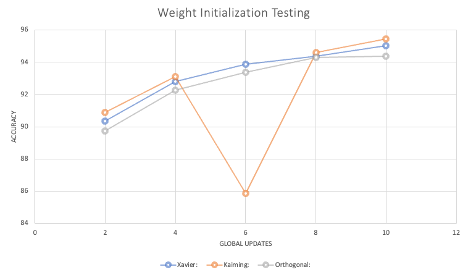
\includegraphics[width=165mm]{thesis/img/tool_select_1.png}
        \caption{Xavier, Kaiming \& Orthogonal Weight Initialization Schemes}
        \label{fig:test_3}
    \end{figure}
    
    \begin{figure}
        \centering
        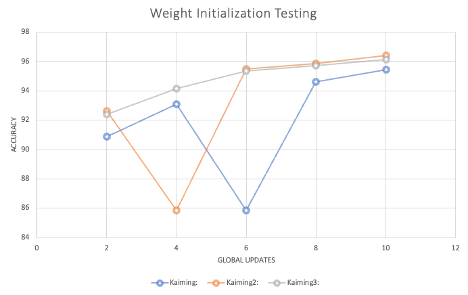
\includegraphics[width=165mm]{thesis/img/tool_select_2.png}
        \caption{Kaiming Scheme Tests for Consistency}
        \label{fig:test_k}
    \end{figure}
    
    \begin{figure}
        \centering
        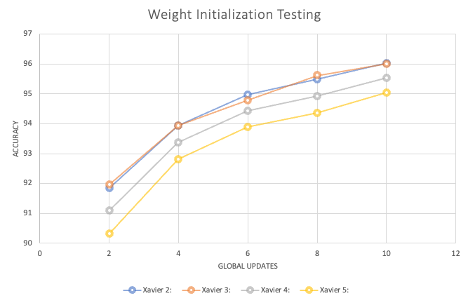
\includegraphics[width=165mm]{thesis/img/tool_select_3.png}
        \caption{Xavier Scheme Tests for Consistency}
        \label{fig:test_x}
    \end{figure}
\end{document}
